\chapter{Experiment Simulation}
\label{ch:Simulation}

Simulated data, or Monte Carlo (MC), plays a very important role in the \nova~analyses. The FD only expects $O(10^2)$ events per year, not nearly enough statistics to fine tune things like selection cuts. Furthermore, it is important that actual parameter measurements use an independent sample of data from that used to train and tune an anlysis. MC solves both of these problems by being explicitly different from the real data and having only computer memory limit statistics.

The full simulation chain is very long and comprises multiple steps, which reduces complexity and provides more opportunity for validation. At every step, the information from previous pieces of the simulation chain are kept so it is always possible to reproduce future results and trace any errors that may occur. The simulation chain consists of two main components, simulation of the beam and the detector response. This chapter discusses both of these areas in more detail, and finishes with a discussion of packages designed to study and validate the results.

\section{Flux Simulation}
\label{sec:SimFlux}

The first main simulation segment is the simulation of the NuMI beam, or the flux simulation. This section starts with the interaction of protons in the target and ends with experiment independent flux files full of neutrino rays that most importantly contain the flavor, direction, energy, and momentum of the neutrinos.

The flux simulation is performed using the FLUGG package, an interface between FLUKA \cite{ref:Fluka1, ref:Fluka2} and Geant4 \cite{ref:Geant41, ref:Geant42}. The version used for the analysis in this dissertation was FLUGG 2009.3, combining FLUKA2011 and Geant4 v4.9.6.p03(c). The FLUKA package is designed to simulate particle interactions and was used to simulate the proton interactions in the target. Geant4 is a toolkit for simulation of particles propagating through matter, and is used in this context to propagate the target interaction products through a detailed model of the NuMI beam line. This model of the beam includes all of the elements discussed in section \ref{sec:NuMI}, starting from the target hall all the way through the rock before the detector halls. The second focusing horn, a representative component of the geometry model, is shown in figure \ref{fig:GeomHorn}.
\begin{figure}[htb]
  \centering
  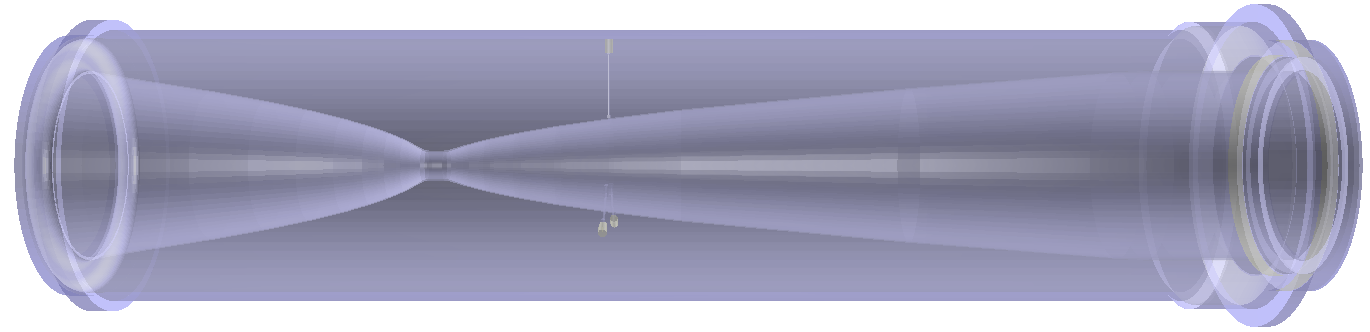
\includegraphics[width=0.9\textwidth]{figures/Horn2.png}
  \caption[Model of the Second Focusing Horn]{Visualization of the geometry used to model the second horn. This image was made during efforts to correctly position the three spider supports seen near the center of the schematic. Figure from \cite{ref:GeomNuMI}.}
  \label{fig:GeomHorn}
\end{figure}

The output of the FLUGG simulation is a set of flugg format flux files. These include the information described at the beginning of this section, but have several other key features as well. Simulating the particle products of every target interaction is extremely expensive on computing resources, so not every particle is tracked. Instead, similar neutrinos are often dropped in lieu of a single entry that is given a greater {\em importance weight}, one of two weights stored in the flux files. The information about the neutrino parent is also stored in the files, including the particle type, energy, momentum, and decay point. This affords later simulation steps the ability to ``redecay'' a neutrino ray to a specific location and calculate the relative probability that this would occur. The latter value is stored as a {\em propagation weight}. Retaining the parent information also allows for event reweighting based on hadronic model studies.

The next piece of the flux simulation is largely a repackaging or the flugg format flux files into a unified format, called Dk2Nu \cite{ref:Dk2Nu}. FLUGG is certainly not the only flux generator, and \nova~is not the only experiment that uses the NuMI beam line. The Dk2Nu format is unified in the sense that it has the same format regardless of flux generator, and valid for any experiment using the NuMI beam.

Dk2Nu format flux files (or simply dk2nu files) are one of the main outputs from the flux simulation. However, one last step is taken to further simplify computation time for later simulation steps. The entries in the dk2nu files are sampled over a `window' that shadows the detector of interest, resulting only in a set of neutrino rays that could create interactions within the detector. The output files from this final step are in the GSimpleNtpFlux format, or more simply referred to as gsimple files \cite{ref:gsimple}.

\section{Detector Simulation}
\label{sec:SimDet}

The second main section in the simulation chain is the detector simulation. This section begins with neutrino interactions, models many different detector response effects, and finishes with files of simulated raw hits, or the signals read out by the detector electronics. The latter portion of this section closely follows the \nova~Simulation Technical Note \cite{ref:TNDetSim}, which provides more detail and further references.

%\subsection{Neutrino Interactions}
%\label{sec:SimGENIE}

Neutrino interactions are modeled using the GENIE event generator product \cite{ref:GENIEGen, ref:GENIE}. For the analysis in this dissertation, version v2.10.4 was used. GENIE requires as input flux files, a model of the detector geometry, and cross section information, and from this determines if and where a neutrino interaction occurs, the type of interaction, and the kinematics of the interaction products. The generator uses a sophisticated model of the nucleus that allows for quasi-elastic, resonant, or deep inelastic scattering, taking into account any intranuclear scattering that may occur after the initial interaction takes place. The output of a GENIE interaction is a list of primary particles that escape the target nucleus and the relevant kinematic variables that describe each entry.

The GENIE output is next fed back to Geant4 for particle propagation through the detector geometry \cite{ref:Geant41, ref:Geant42}. It models the primary particles interactions within the detector, including energy deposition and secondary interactions. The physical processes considered and modeled are somewhat configurable via the choice of the physics list. At this point in the simulation, it is much more important to accurately track the detailed interactions, so particles are not dropped as in the flux simulation; instead, a more precise model was used here. The specific physics list used was QGSP\_BERT\_HP, where QGSP specifies that high energy hadrons ($> 10\unit{GeV}$) are modeled with the quark gluon string model, BERT speficies that lower energy hadrons ($< 10\unit{GeV}$) are modeled with the Bertini cascade model, and HP toggles the usage of a high precision neutron model that tracks low energy neutrons ($< 20\unit{MeV}$) \cite{ref:TNDetSim}. The output from Geant4 at this stage is a list particles involved in the detector interaction and a full suite of information about each one, called the MC truth. The information that is most important to the next simulation step is a list of energy depositions and positions.

It is worth noting that the simulated events for the Near and far Detectors are generated somewhat differently. The FD expects a very low event rate per beam spill, while the ND expects multiple events per spill. As a result, the FD events are generated one at a time with the simulation calculating the POT needed for the event occur, and ND events are generated assuming a constant POT/spill and a variable number of events. Furthermore, the high rate of interactions at the ND means that it observes many muons that originate from neutrino interactions that begin in the rock outside of the detector. Most of these so called rock events do not result in any detector activity, so tracking them wastes valuable computing time. To deal with this, the ND detector events and single rock events are generated separately, and only the rock events that cause detector activity are kept. The final ND event records are made by overlaying rock events on the detector events. The number of rock singles to overlay is drawn from a Poisson distribution with a mean determined from data \cite{ref:SimRock}.

Geant4 also handles the next piece of the simulation, the conversion between energy deposition and light yield. For low energies, the rate of light produced in liquid scintillator is proportional to the energy deposition, but the light yield begins to quench for particles with high enough energies. The Birks-Chou Law, encapsulated within a Geant4 module, is used to model the relationship between scintillator light yield rate, $\frac{dL}{dx}$, and particle energy deposition rate, $\frac{dE}{dx}$ \cite{ref:BirksChou}.

\beq
\frac{dL}{dx} = L_0 \frac{ \frac{dE}{dx} }{1 + k_B \frac{dE}{dx} + k_C \left( \frac{dE}{dx} \right)^2} 
\label{eq:BirksChou}
\eeq

\n Above, the constants $L_0$, $k_B$, and $k_C$ are dependent on the scintillator material and had to be estimated for \nova~as no measurement existed for the particular materials used in the experiment. A study was performed comparing the energy deposition at the end of proton tracks in the ND for both data and MC to find parameters that would generate agreement between the two \cite{ref:DanBirks}. The results of the study were $k_B = 0.04\unit{cm/MeV}$ and $k_C = -0.0005\unit{(cm/MeV)}^2$. The output from this simulation step is a set of energy depositions now encoded as light yield called FLSHits, or fiber in liquid scintillator hits.

%\subsection{Photon Propagation}
%\label{sec:Photon}

The next part of the simulation simulates the capture of the scintillation photons, their transport through the WLS fiber to the electronics, and their conversion into photoelectrons after collection by the APD. The detector is treated as uniform for this section, with the assumption that any individual differences between cells would be removed by the downstream calibration. Individual photons are not traced from emission to the electronics due to its expensive computation time, despite the ability of Geant4 to perform this simulation. Rather, a template that parametrizes the photon transport are created and individual results are drawn from this.

The first template is a collection rate of photons by the WLS fibers as a function of time from scintillator emission and distance along the cell length from scintillator emission. The template is constructed using a ray tracing algorithm that considers a photon to be captured when it intersects with a fiber.  The mean number of photons per energy deposited is a tunable parameter that is constrained using cosmic ray data. The scintillator emission spectrum and cell wall reflectivity are modeled as a function of wavelength based on data from \nova's quality control database.

Next, the photons are transported through the fiber to the electronics. Since the fiber is looped and both ends are read out, half of the photons are transported to each end. The number of photons that reach the fiber ends is attenuated by applying an attenuation curve derived from quality control tests as a function of distance from the fiber end. Another template is constructed using a ray tracer that models transport time as a function of distance. The actual transport times are drawn from this template instead of handling the photon capture angles individually.

At this point in the simulation, there is a number of photons that reach the APD as a function of time. This is converted to photoelectrons (PEs) assuming a flat quantum efficiency of $0.85$ for every APD. The exact number of PEs collected is drawn from a log-normal distribution with a mean of the expected number of PEs to account for the repeated random charge avalanche process within the APD. The final output of the photon transport simulation is a set of objects that encodes the number of PEs as a function of time, called PhotonSignals.

%\subsection{Electronic Readout}
%\label{sec:Electronics}

The last piece of the detector simulation models the electronics readout. This section starts with the number of PEs collected by the APDs and simulates the effects of the electronics to generate the raw signals equivalent to data. There are three main chips on the FEBs simulated here, an application-specific integrated circuit (ASIC) that performs the initial pulse shaping, an analog to digital converter (ADC) that samples each channel periodically, and a field-programmable gate array (FPGA) that searches for peaks above noise threshold using a dual correlated sampling trace. Before digitizing the signal by the ADC, two additional data driven effects are simulated. First, noise hits are added before the sample is digitized by drawing from a histogram of noise from cosmic data. The second effect is APD sag, or the tendency when one APD channel observes a large hit for other channel baselines to slightly drop. After these effects are applied and the signal is digitized, the ADC values of the hits above threshold are the final output of the detector simulation and are recorded as a vector of objects called RawDigits. This is the lowest level object that has the same format for both data and MC; however, the additional truth information is always stored for the MC for validation and further studies.

%\subsection{Detector Conditions}
%\label{sec:Masking}

In real data, readout did not always occur from every cell in the full detector. Full diblocks sometimes were missing due to original commissioning or repair work. Within individual diblocks, single channels can be masked off for too high noise levels or too low data rates. The diblock configuration for data was stored by run, and the channel masks were stored by subrun. To most accurately reflect the detector running conditions, the MC was generated matching the configurations in data, or weighting the MC configurations simulated by POT.

%\subsection{Oscillations and File Format}
%\label{sec:FluxSwap}

The FD MC files generated do not include any realistic oscillation probabilities; instead, three sets of files are produced. The first set assumes that there are no oscillations, called nonswap files. These files are consist of the same percentage of $\numu$ and $\nue$ generated naturally in the NuMI beam. The simulation does not generate any $\nutau$ so these events are entirely absent from nonswap files. The second set of files, called fluxswap, completely oscillate all $\numu$ to $\nue$, and vice versa. Finally, the third set of files, called tauswap, completely oscillate all $\numu$ and $\nue$ to $\nutau$. All three files include the same rate of NC events. Oscillation weights as a function of true energy can be applied individually to each interaction channel at a later stage, which allows for realistic conditions that can also be tuned without generating entirely new MC.

\section{Validation}